\documentclass[11pt, a4paper]{article}
\usepackage{pdfpages}
\usepackage{parallel}
\usepackage[T2A]{fontenc}
\usepackage{ucs}
\usepackage[utf8x]{inputenc}
\usepackage[polish,english,russian]{babel}
\usepackage{hyperref}
\usepackage{rotating}
\usepackage[inner=2cm,top=1.8cm,outer=2cm,bottom=2.3cm,nohead]{geometry}
\usepackage{listings}
\usepackage{graphicx}
\usepackage{wrapfig}
\usepackage{longtable}
\usepackage{indentfirst}
\usepackage{array}
\usepackage{tikzsymbols}
\usepackage{soul}
\usepackage[ruled,vlined]{algorithm2e}
%\counterwithout{figure}{section} 

\usepackage{url}
\makeatletter
\g@addto@macro{\UrlBreaks}{\UrlOrds}
\makeatother

\newcolumntype{P}[1]{>{\raggedright\arraybackslash}p{#1}}
\frenchspacing
\usepackage{fixltx2e} %text sub- and superscripts
\usepackage{icomma} % коскі ў матэматычным рэжыме
\PreloadUnicodePage{4}

\newcommand{\longpage}{\enlargethispage{\baselineskip}}
\newcommand{\shortpage}{\enlargethispage{-\baselineskip}}

\def\switchlang#1{\expandafter\csname switchlang#1\endcsname}
\def\switchlangbe{
\let\saverefname=\refname%
\def\refname{Літаратура}%
\def\figurename{Іл.}%
}
\def\switchlangen{
\let\saverefname=\refname%
\def\refname{References}%
\def\figurename{Fig.}%
}
\def\switchlangru{
\let\saverefname=\refname%
\let\savefigurename=\figurename%
\def\refname{Литература}%
\def\figurename{Рис.}%
}

\hyphenation{admi-ni-stra-tive}
\hyphenation{ex-pe-ri-ence}
\hyphenation{fle-xi-bi-li-ty}
\hyphenation{Py-thon}
\hyphenation{ma-the-ma-ti-cal}
\hyphenation{re-ported}
\hyphenation{imp-le-menta-tions}
\hyphenation{pro-vides}
\hyphenation{en-gi-neering}
\hyphenation{com-pa-ti-bi-li-ty}
\hyphenation{im-pos-sible}
\hyphenation{desk-top}
\hyphenation{elec-tro-nic}
\hyphenation{com-pa-ny}
\hyphenation{de-ve-lop-ment}
\hyphenation{de-ve-loping}
\hyphenation{de-ve-lop}
\hyphenation{da-ta-ba-se}
\hyphenation{plat-forms}
\hyphenation{or-ga-ni-za-tion}
\hyphenation{pro-gramming}
\hyphenation{in-stru-ments}
\hyphenation{Li-nux}
\hyphenation{sour-ce}
\hyphenation{en-vi-ron-ment}
\hyphenation{Te-le-pathy}
\hyphenation{Li-nux-ov-ka}
\hyphenation{Open-BSD}
\hyphenation{Free-BSD}
\hyphenation{men-ti-on-ed}
\hyphenation{app-li-ca-tion}

\def\progref!#1!{\texttt{#1}}
\renewcommand{\arraystretch}{2} %Іначай формулы ў матрыцы зліпаюцца з лініямі
\usepackage{array}

\def\interview #1 (#2), #3, #4, #5\par{

\section[#1, #3, #4]{#1 -- #3, #4}
\def\qname{LVEE}
\def\aname{#1}
\def\q ##1\par{{\noindent \bf \qname: ##1 }\par}
\def\a{{\noindent \bf \aname: } \def\qname{L}\def\aname{#2}}
}

\def\interview* #1 (#2), #3, #4, #5\par{

\section*{#1\\{\small\rm #3, #4. #5}}
\ifx\ParallelWhichBox\undefined%
    \addcontentsline{toc}{section}{#1, #3, #4}%
\else%
\ifnum\ParallelWhichBox=0%
    \addcontentsline{toc}{section}{#1, #3, #4}%
\fi\fi%

\def\qname{LVEE}
\def\aname{#1}
\def\q ##1\par{{\noindent \bf \qname: ##1 }\par}
\def\a{{\noindent \bf \aname: } \def\qname{L}\def\aname{#2}}
}

\newcommand{\interviewfooter}[1]{
\vskip 1em
\noindent \textit{#1}
}


\begin{document}

\title{1986 "--- NEC Crystal mouse}
\date{}
\maketitle

    В сентябре 1986 года NEC анонсировала рабочую станцию EWS 4800, оснащенную ОС UNIX и центральным процессором на базе архитектуры CISC (компьютер со сложным набором команд). Эта машина была спроектирована как рабочая станция для инженеров, для повышения эффективности решения таких задач, как разработка программного обеспечения, автоматизированное проектирование, научные и инженерные вычисления, сбор и анализ экспериментальных данных.
    
    Эта рабочая станция позволяла комплексно использовать все типы данных: текст, рисунки, изображения, видео и аудио. Она была оснащена графическим многооконным интерфейсом и выделенным высокоскоростным графическим процессором, который позволял отрисовывать с высокой скоростью 75 000 векторов в секунду и обрабатывать до 48 окон. В комплект входил также большой 20-дюймовый дисплей с разрешением 1280 на 1024 точки и 256-битной цветностью.
    
    В комплекте с рабочей станцией поставлялась мышь Crystall Mouse. Это оптическое устройство позиционирования, использующее специальный зеркальный коврик. 

\begin{figure}[h]
    \centering
    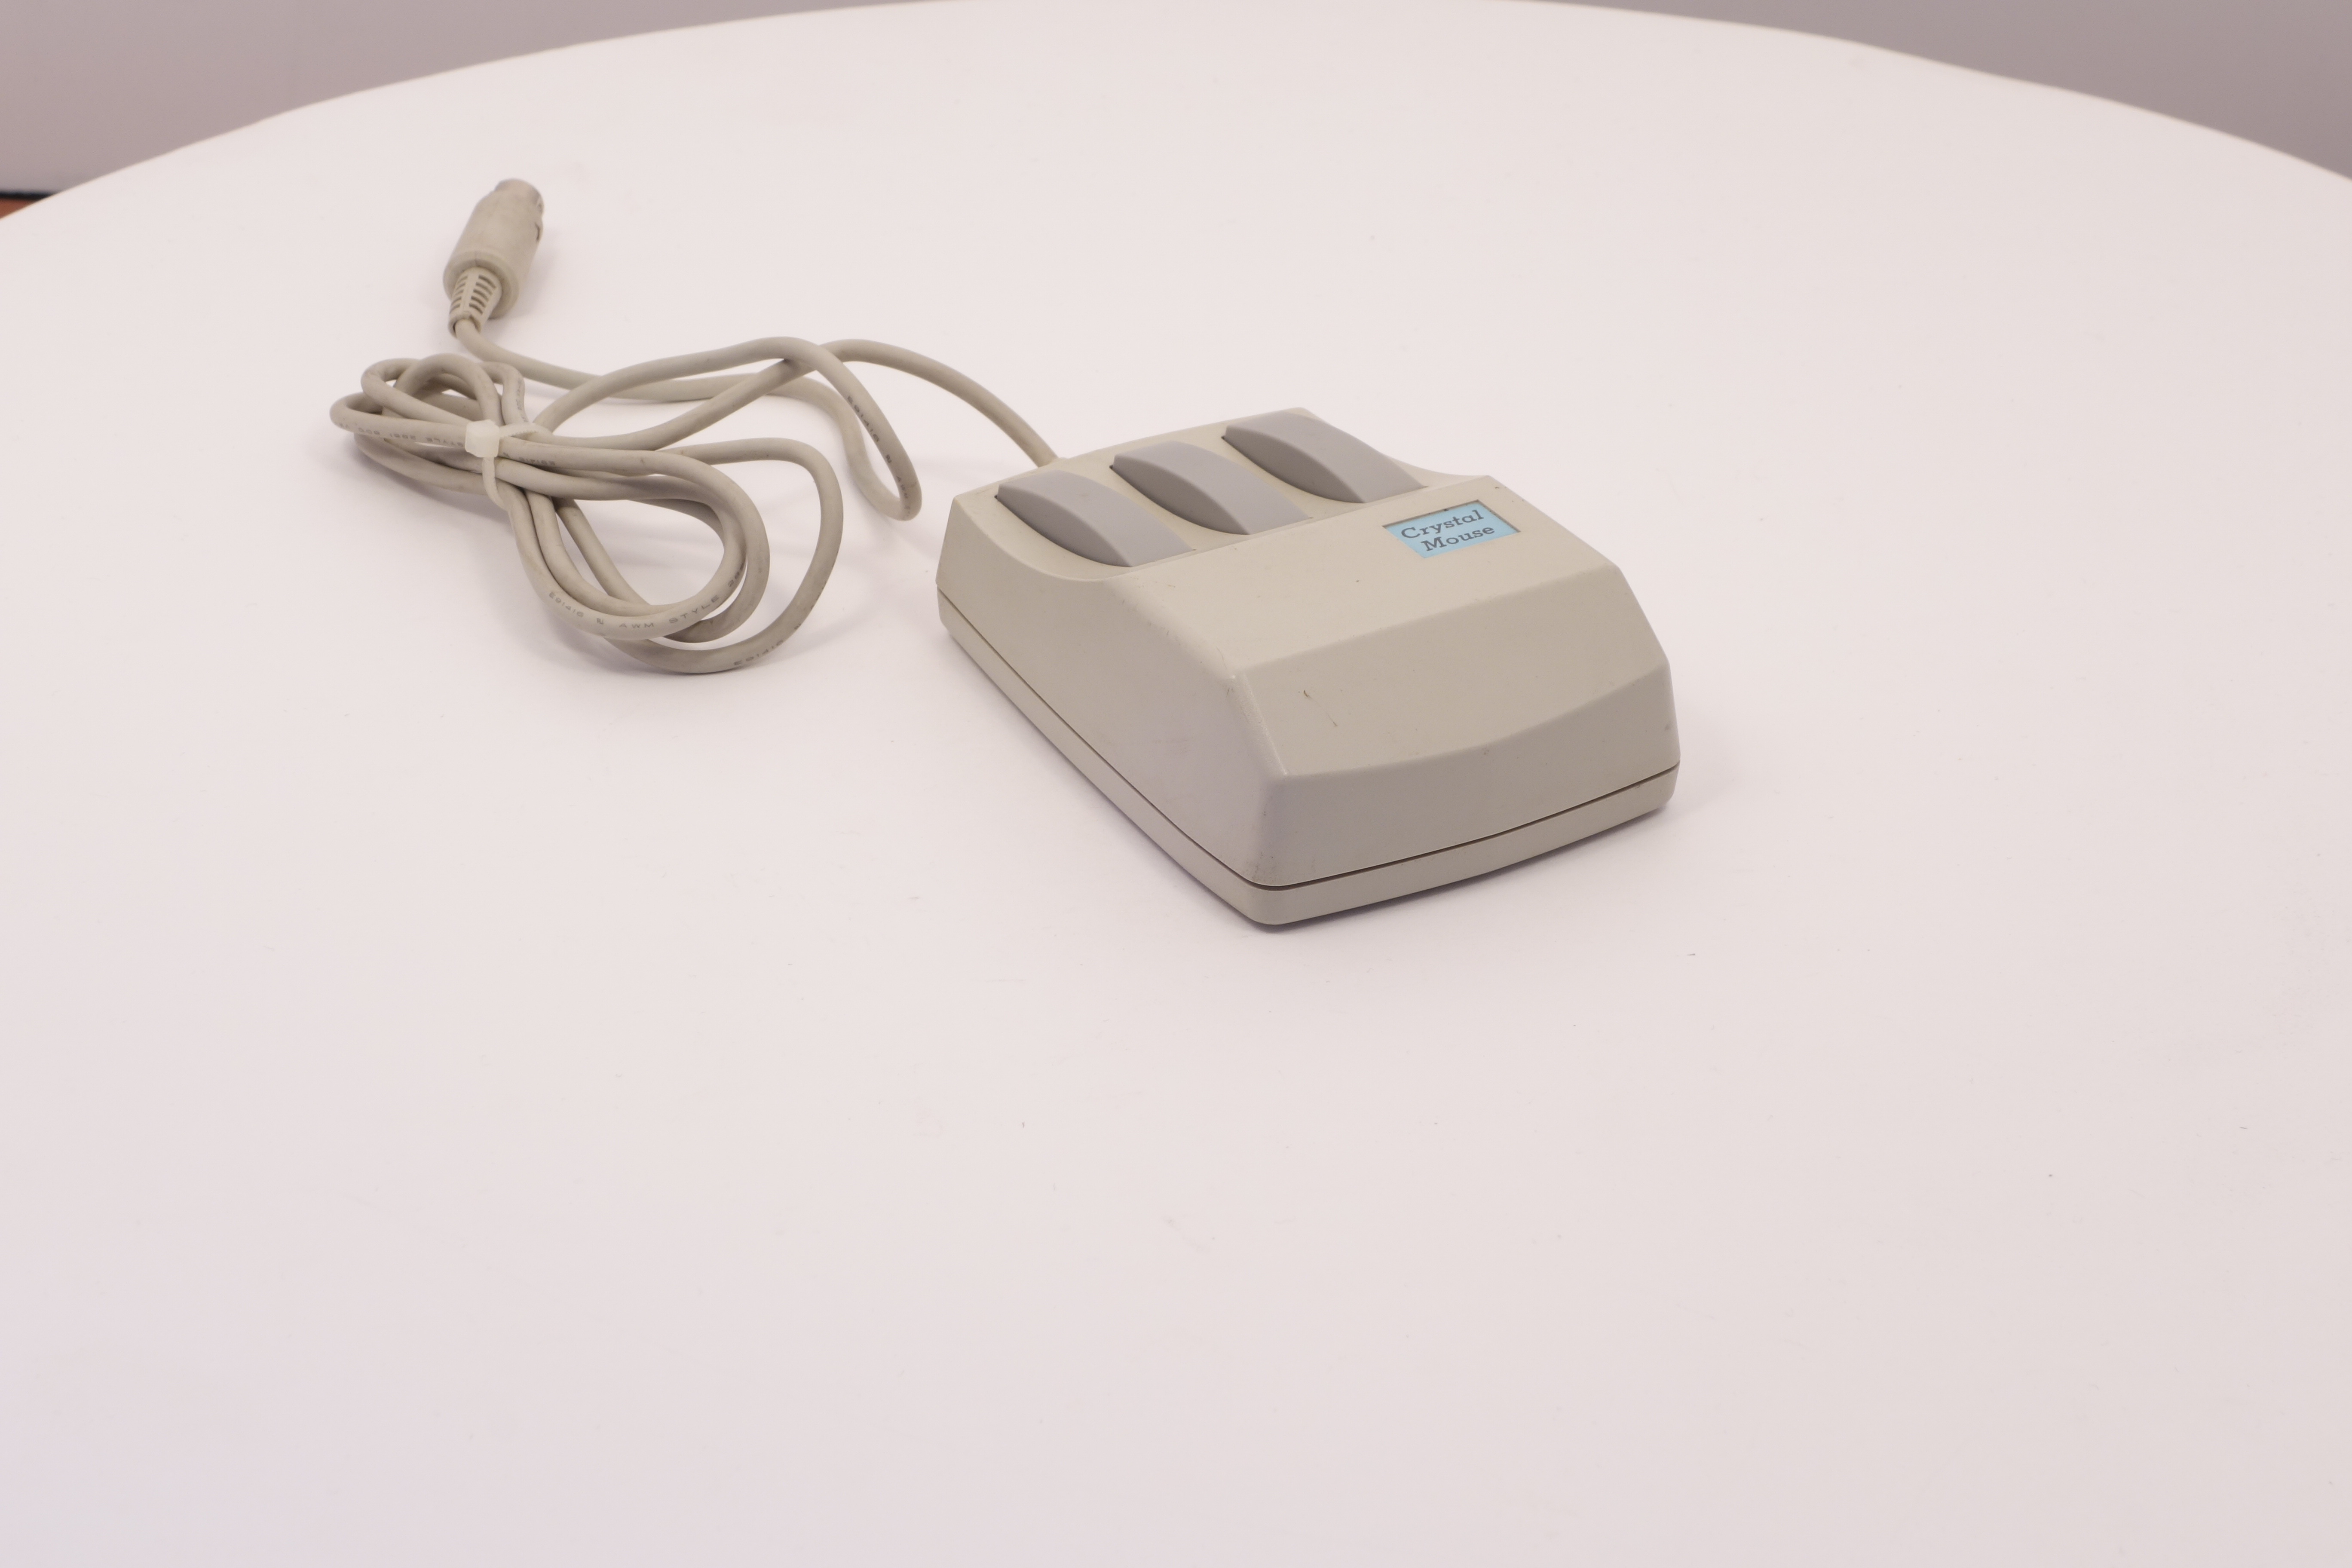
\includegraphics[scale=0.2]{necNorm.jpg}
    \caption{Изображение Crystal Mouse Nec, вид спереди}
    \label{fig:NecCrystalPic}
\end{figure}

\begin{figure}[h]
    \centering
    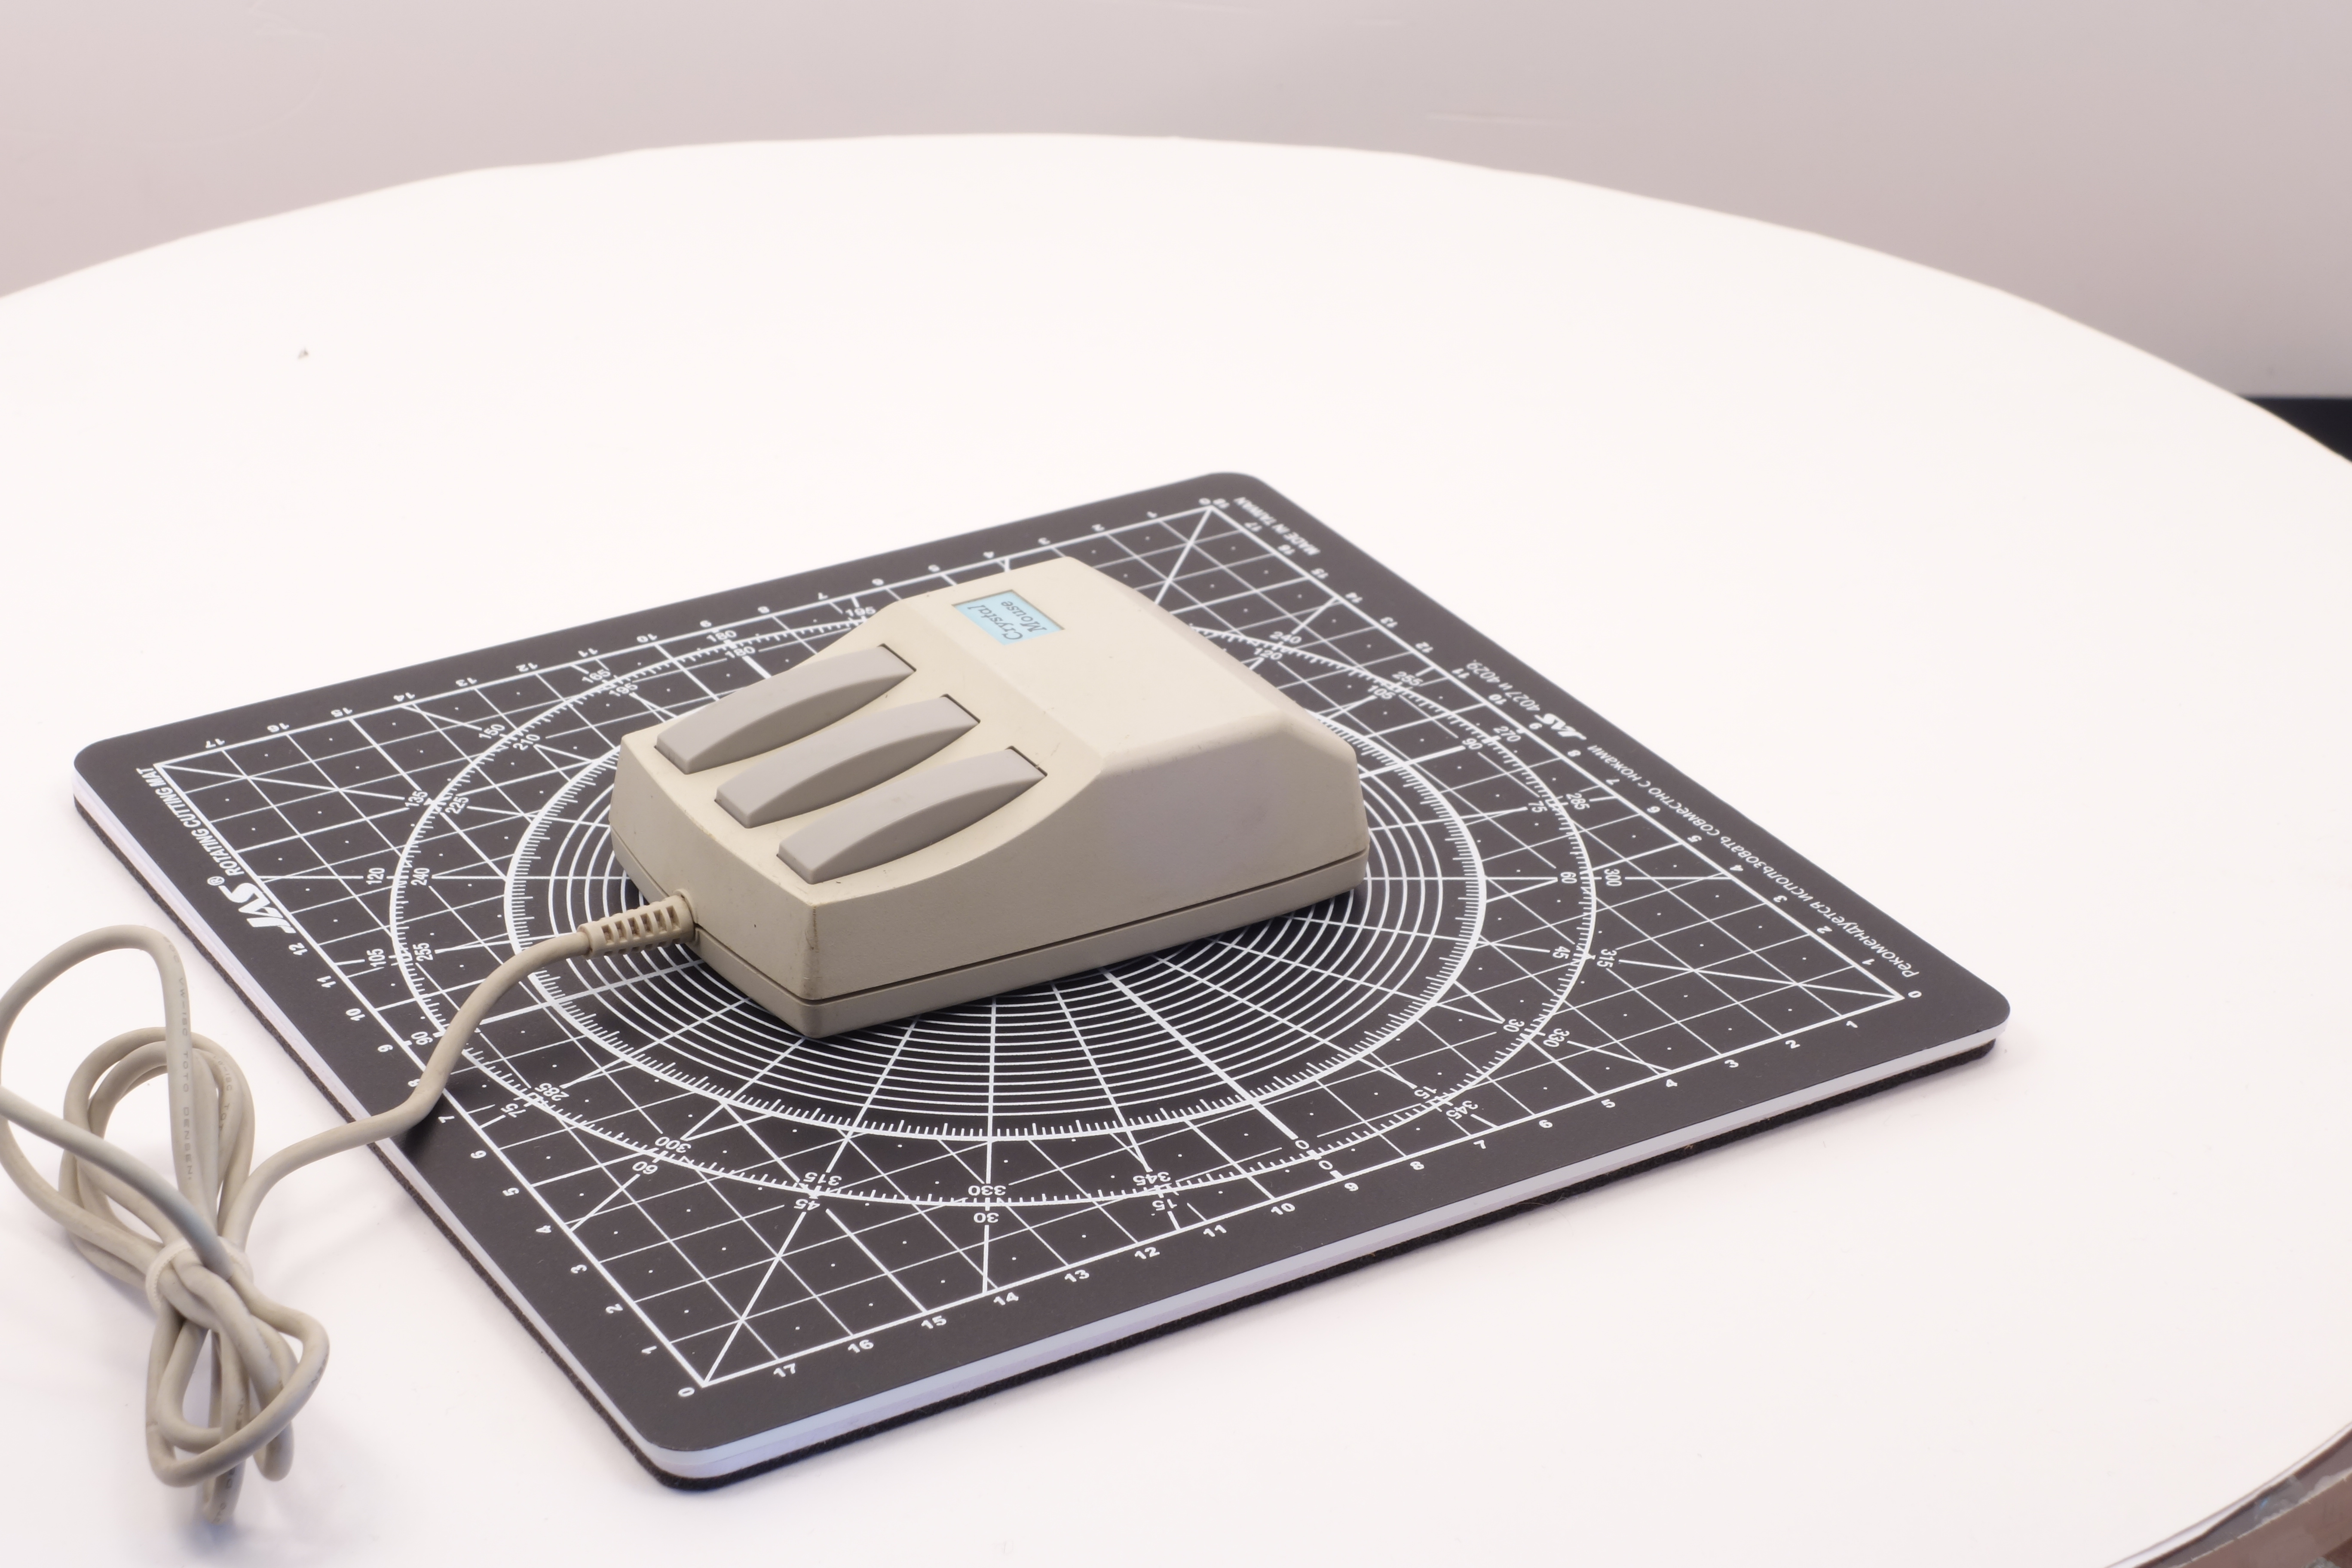
\includegraphics[scale=0.2]{NecKovrik.JPG}
    \caption{Изображение Crystal Mouse Nec на размерном коврике с шагом сетки 1~см}
    \label{fig:NecCrystalSize}
\end{figure}

В плане размера манипулятор представляет собой типичное для 80-х годов оптическое устройство управления курсором. 
    В плане эргномики во внешем виде Crystall Mouse прослеживается ярко выраженный индустриальный дизайн. При этом большое количество углов и плоских граней отчасти компенсируется закругленными стыками граней в ближней к пользователю части корпуса, и выпуклыми продолговатыми кнопками, удобно расположенными в зоне досягаемости пальцев пользователя (рисунок 2.10).

На верхней стенке корпуса выделено название мыши <<Crystal Mouse>> с двумя треугольными стилизованными мышками в очертаниях и сплошных линиях.

\begin{figure}[h]
    \centering
    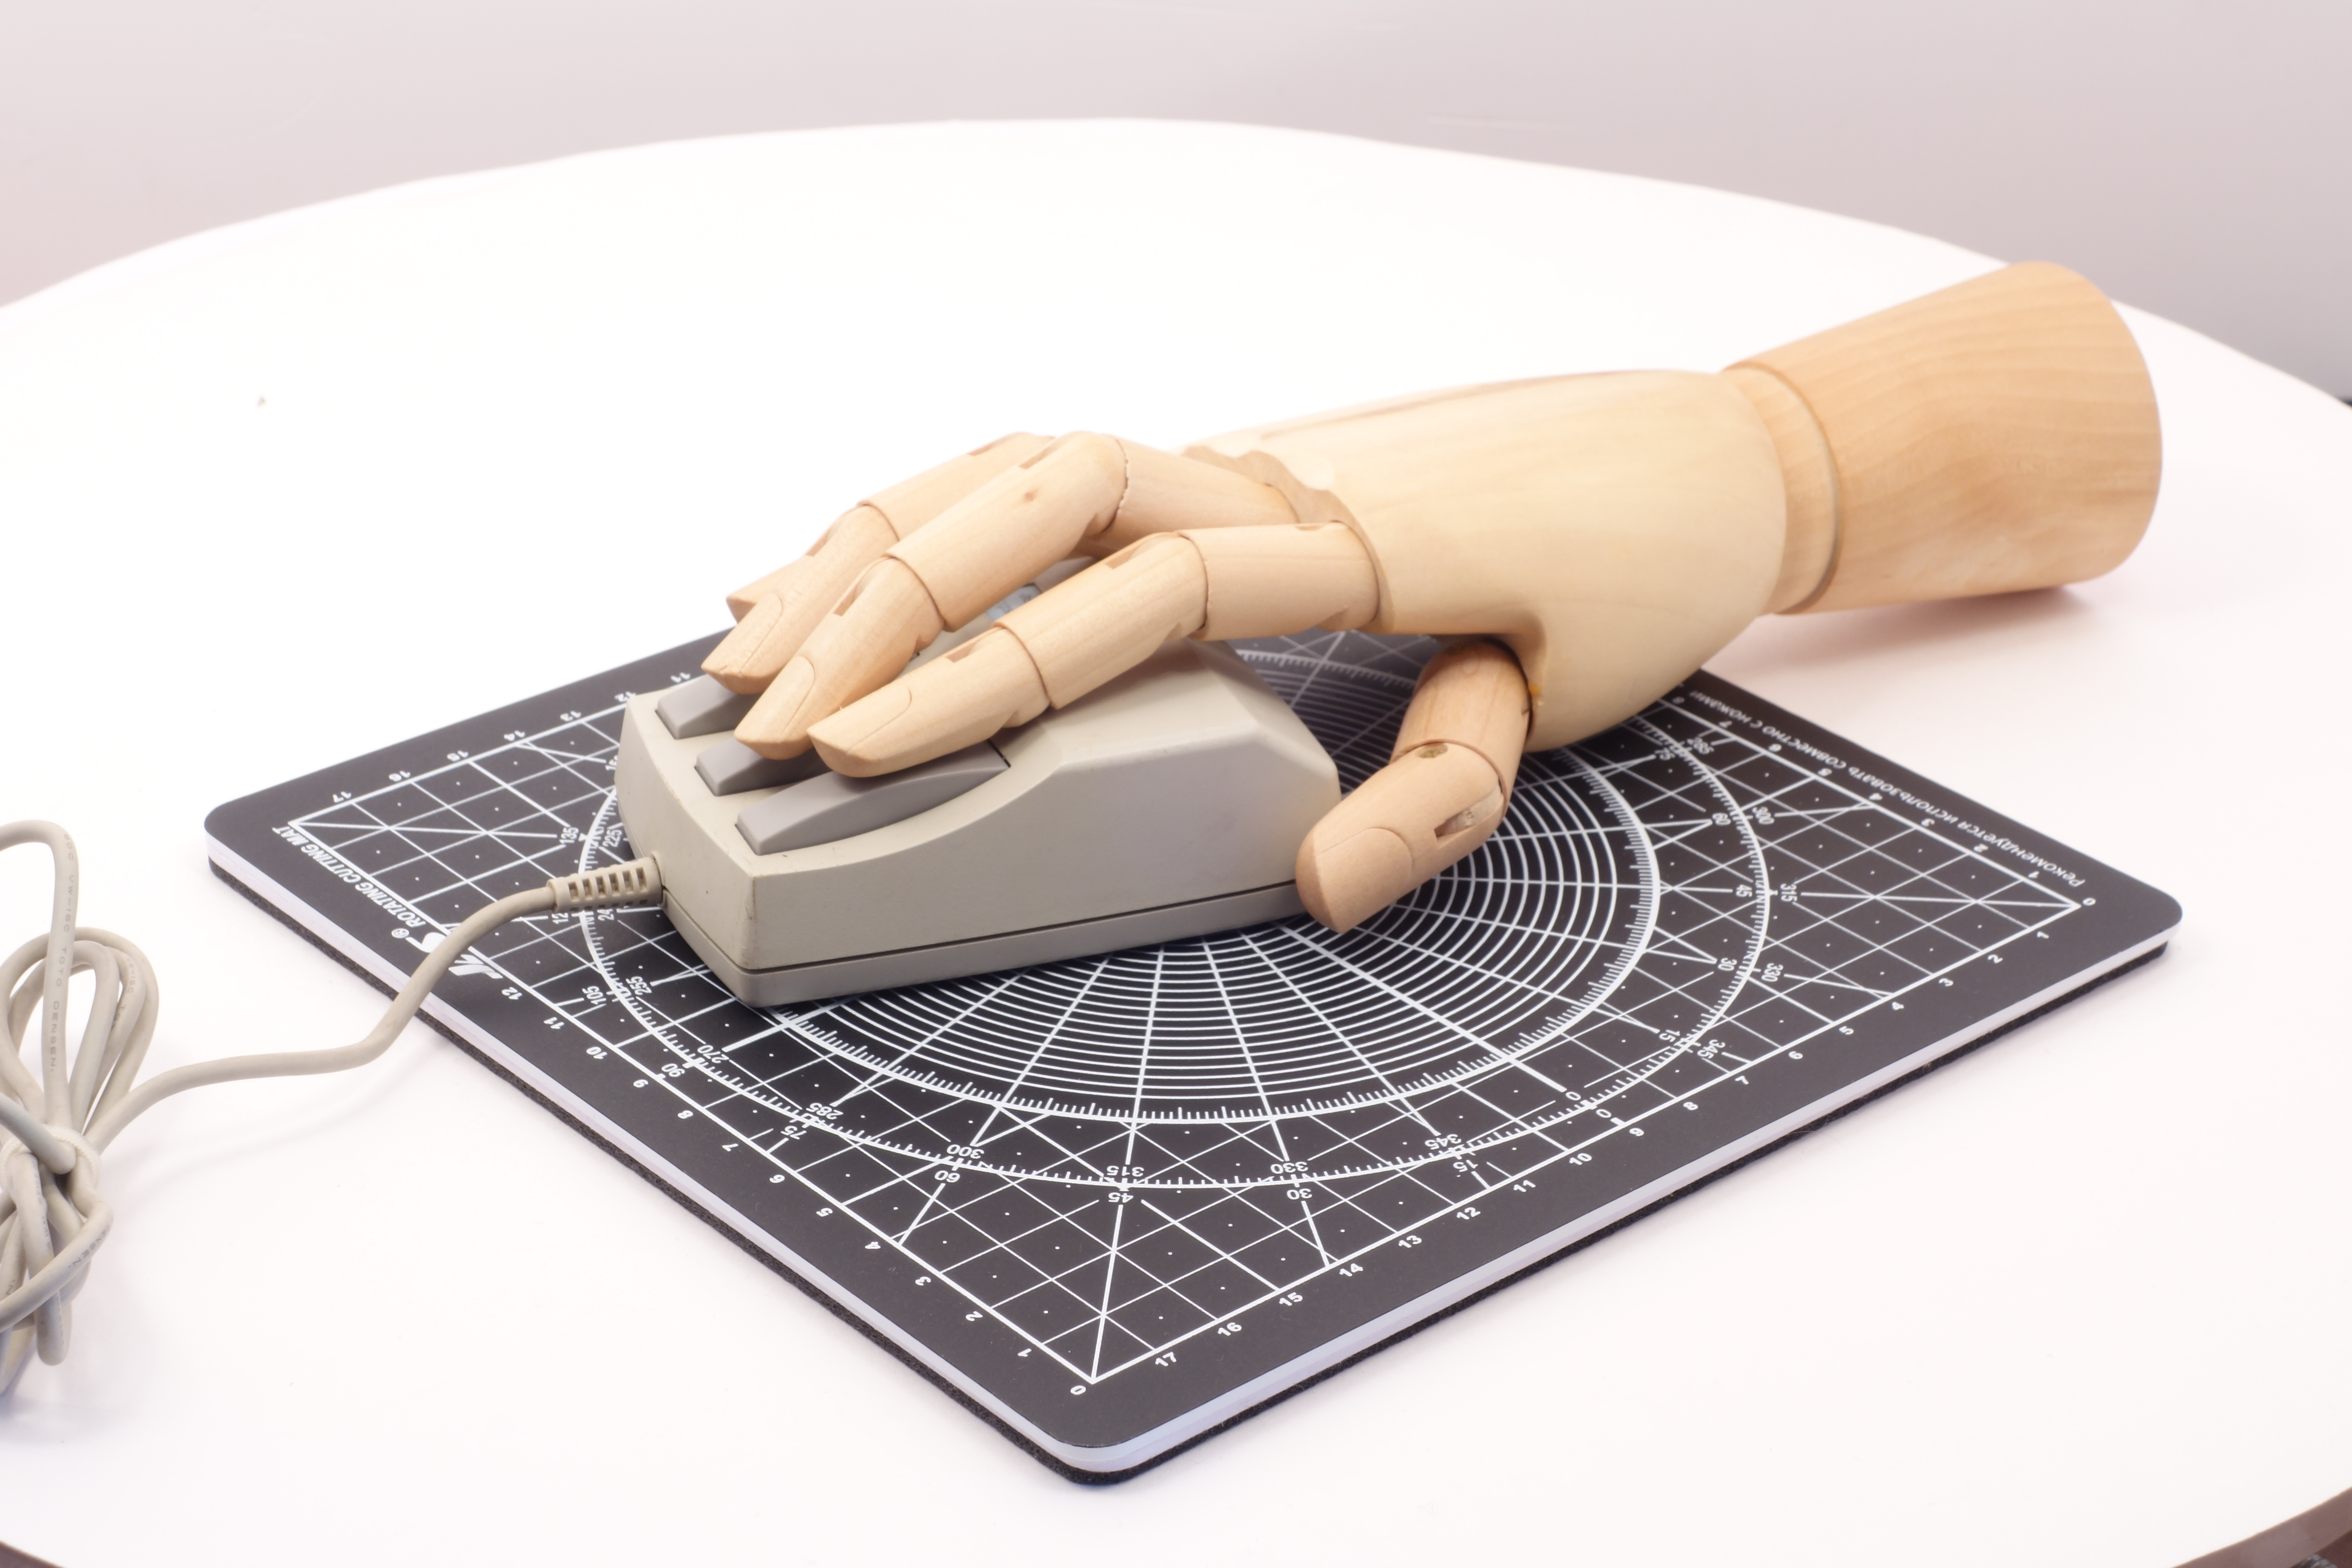
\includegraphics[scale=0.2]{NecRuka.JPG}
    \caption{Crystal Mouse Nec с моделью руки человека}
    \label{fig:NecCrystalHand}
\end{figure}
    
    По интерфейсу подключения Crystall Mouse относится к категории 
    Bus Mouse (шинная мышь). Особенностью таких мышей является то, что обработку сигналов оптопар производит не микросхема в корпусе мыши, а специальный адаптер в системном блоке компьютера. 
    Поэтому мышь питается от компьютера без отдельного блока питания, в отличие от многих ранних оптических моделей, подключавшихся к последовательному порту IBM PC. 

\begin{figure}[h]
    \centering
    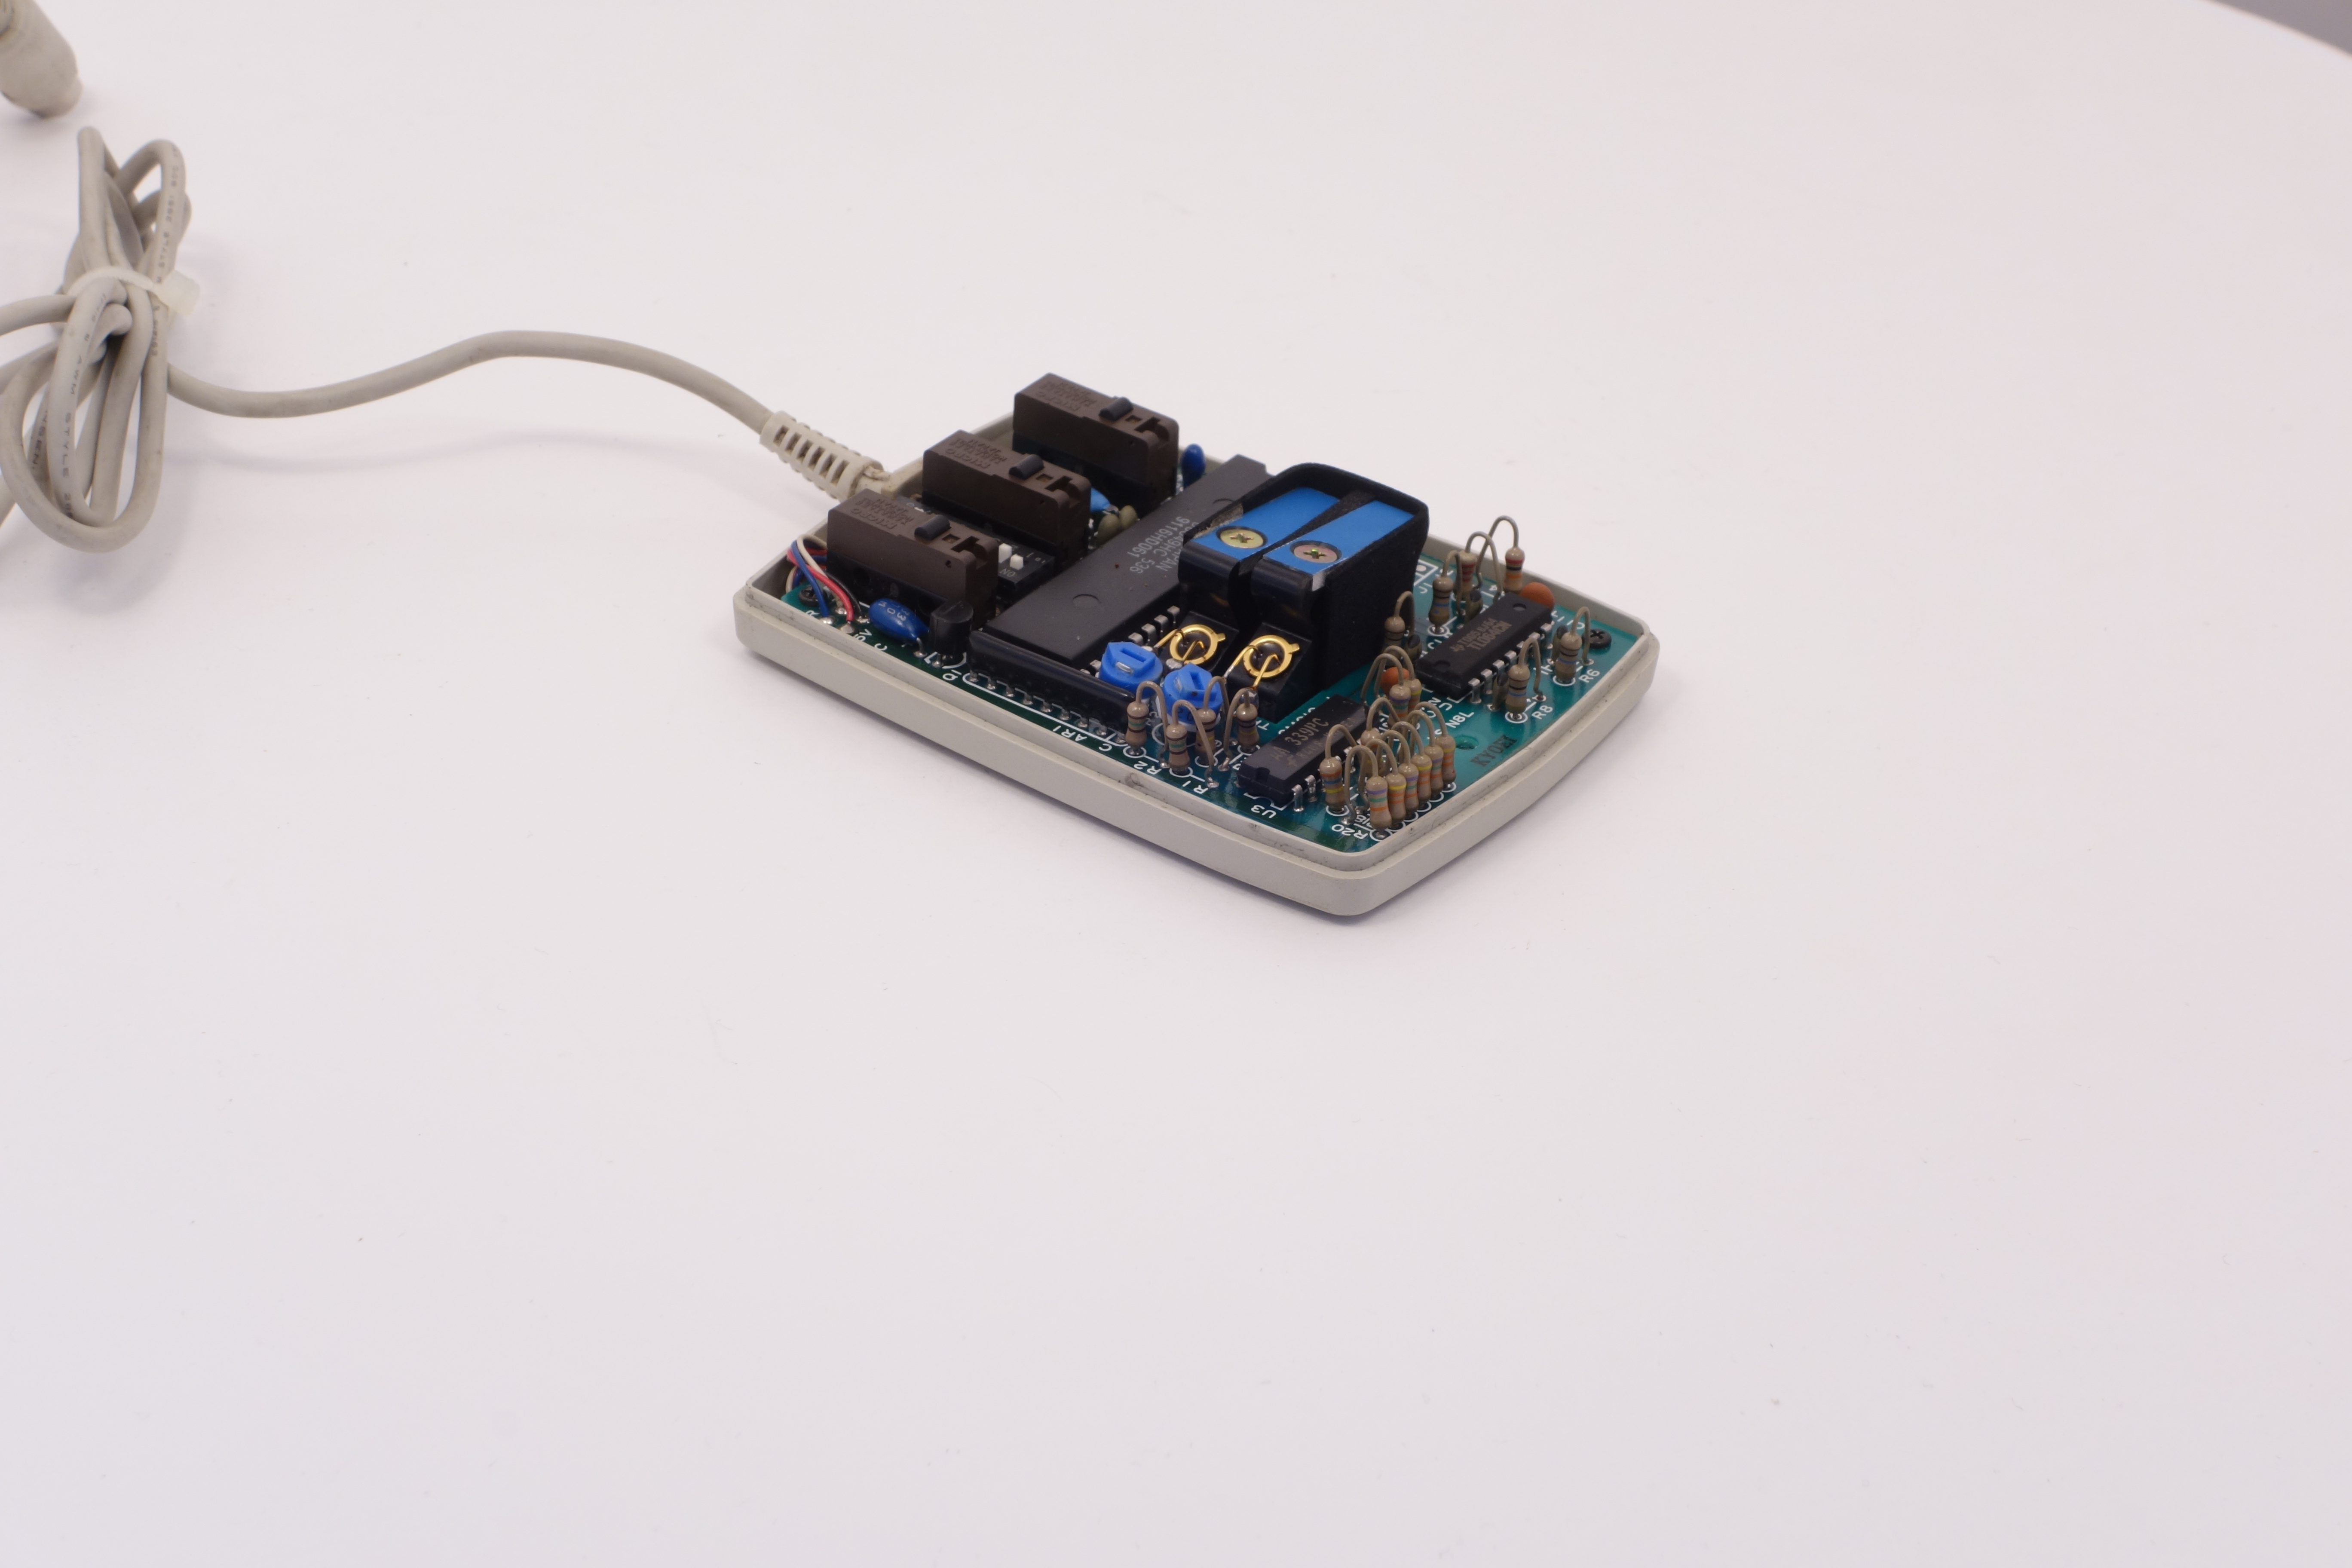
\includegraphics[scale=0.3]{necraz.jpg}
    \caption{Crystal Mouse Nec в разобранном виде}
    \label{fig:NecCrystalInside}
\end{figure}

    В разобранном виде манипулятор показан на рисунке 2.11, где можно увидеть оригинальную конструкцию оптической мыши, соответствующую описанной в п. 2.3, однако в отличие от большинства оптических мышей 80-х годов, не являющейся копией изделия Mouse Systems - первой оптической мыши с зеркальным ковриком, ставшей прототипом для последующих манипуляторов данного типа.
    
\begin{thebibliography}{9}
\bibitem {yt} NEC EWS4800 \url{http://museum.ipsj.or.jp/en/computer/work/0003.html}
\end{thebibliography}
\end{document}
